% -----------------------------------------------------------
\section{Additional experiments}
% ------------------------------------------------------------

This section gives two further comparisons of the original and new versions of lookout, a set of showcase examples, and the details of the bandwidth sensitivity study of Section 4.6 of the main paper. Both versions use the default parameters $\alpha = 0.01$, $\beta = 0.9$ and $\gamma = 0.98$, with scaling applied.

\subsection{Experiment S1: Different anomaly means for Normal distribution}

The non-anomalous observations have independent $\mathcal{N}(0, 1)$ coordinates in $\R^2$, and the anomalies independent $\mathcal{N}(\mu, 1)$ coordinates with $\mu \in \{2.50, 2.75, \dots, 4.00\}$. Each replication has 1000 non-anomalies and 10 anomalies, and there are 20 replications for each value of $\mu$. \cref{fig:expS1} shows the data and results. As $\mu$ increases the anomalies move away from the non-anomalies and the true positive rate rises. The two versions have similar true positive rates at every value of $\mu$. The false positive rate is about 0.008 for the new version and between 0.002 and 0.005 for the original.

\begin{figure}[!hb]
  \centering
  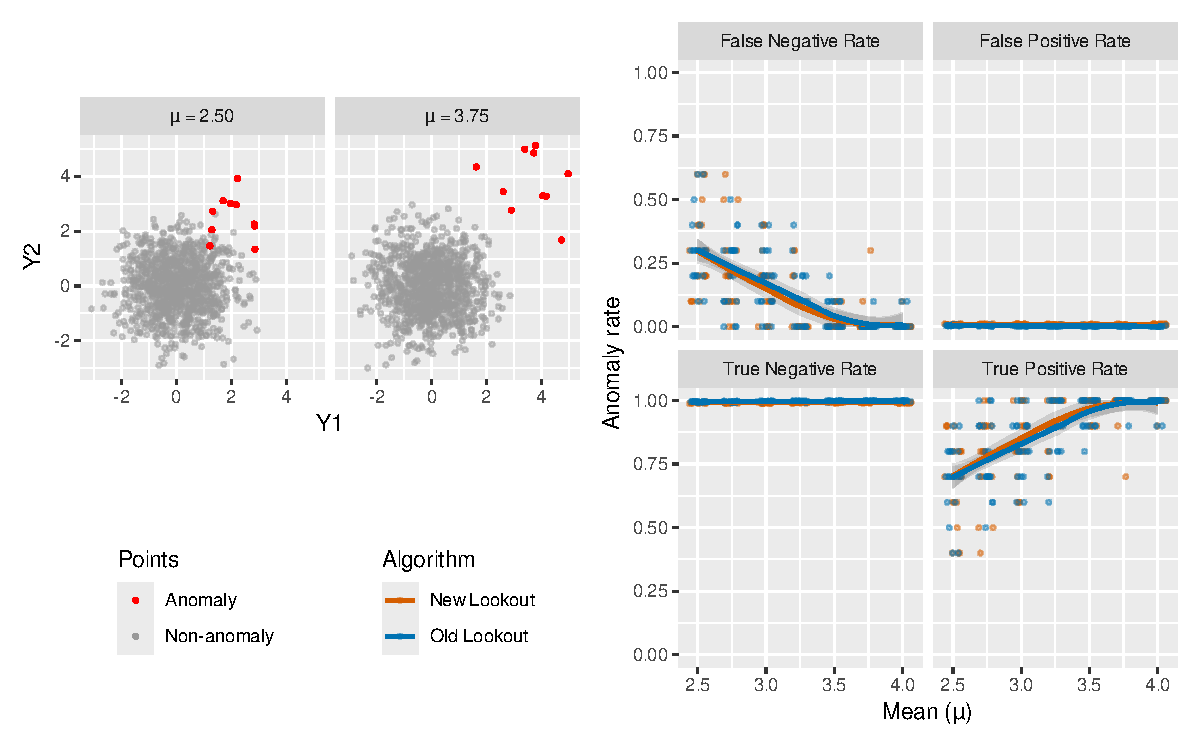
\includegraphics[width=1\textwidth]{Figures/ExpS1_Normal_Rates.pdf}
  \caption{Experiment S1. Left: data with $\mu = 2.5$ and $\mu = 3.75$; anomalies with higher values of $\mu$ are easier to identify. Right: error rates of the two versions of lookout, with points jittered horizontally.}
  \label{fig:expS1}
\end{figure}

\subsection[Experiment S2: Anomalies on the boundary as n increases, Gamma distribution]{Experiment S2: Anomalies on the boundary as $n$ increases, Gamma distribution}

This experiment repeats Experiment 2 of the main paper with gamma-distributed observations. The $n$ non-anomalous observations have independent gamma coordinates in $\R^2$ with shape 2 and rate 2. For the anomalies, we generate $n$ further points with independent gamma coordinates with shape 2.2 and rate 2, keep those whose distance from the origin exceeds the 0.99 quantile of the distances of the non-anomalous observations, and sample $0.005n$ of them. There are 10 replications for each $n \in \{1000, 2000, \ldots, 10000\}$, and the kernel density estimates use the truncated sum with 100 neighbours. \cref{fig:expS2} shows the data for $n = 10000$ and the results. The true positive rate of the new version is between 0.76 and 0.84, and at least as high as that of the original at every $n$. The false positive rate is about 0.012 for the new version and 0.008 for the original.

\begin{figure}[!thb]
  \centering
  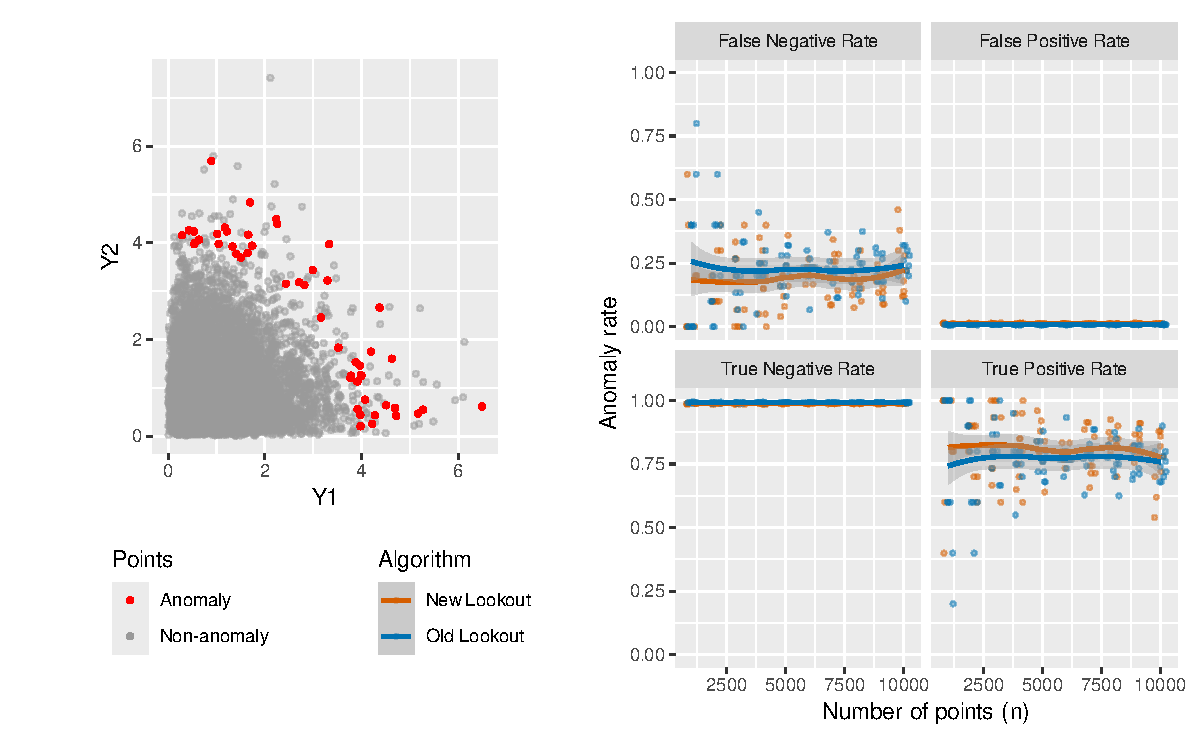
\includegraphics[width=\textwidth]{Figures/ExpS2.pdf}
  \caption{Experiment S2. Left: data for $n=10000$. Right: error rates of the two versions of lookout, with points jittered horizontally.}
  \label{fig:expS2}
\end{figure}

\subsection{Showcase examples}\label{sec:showcase}

\begin{figure}[!p]
  \centering
  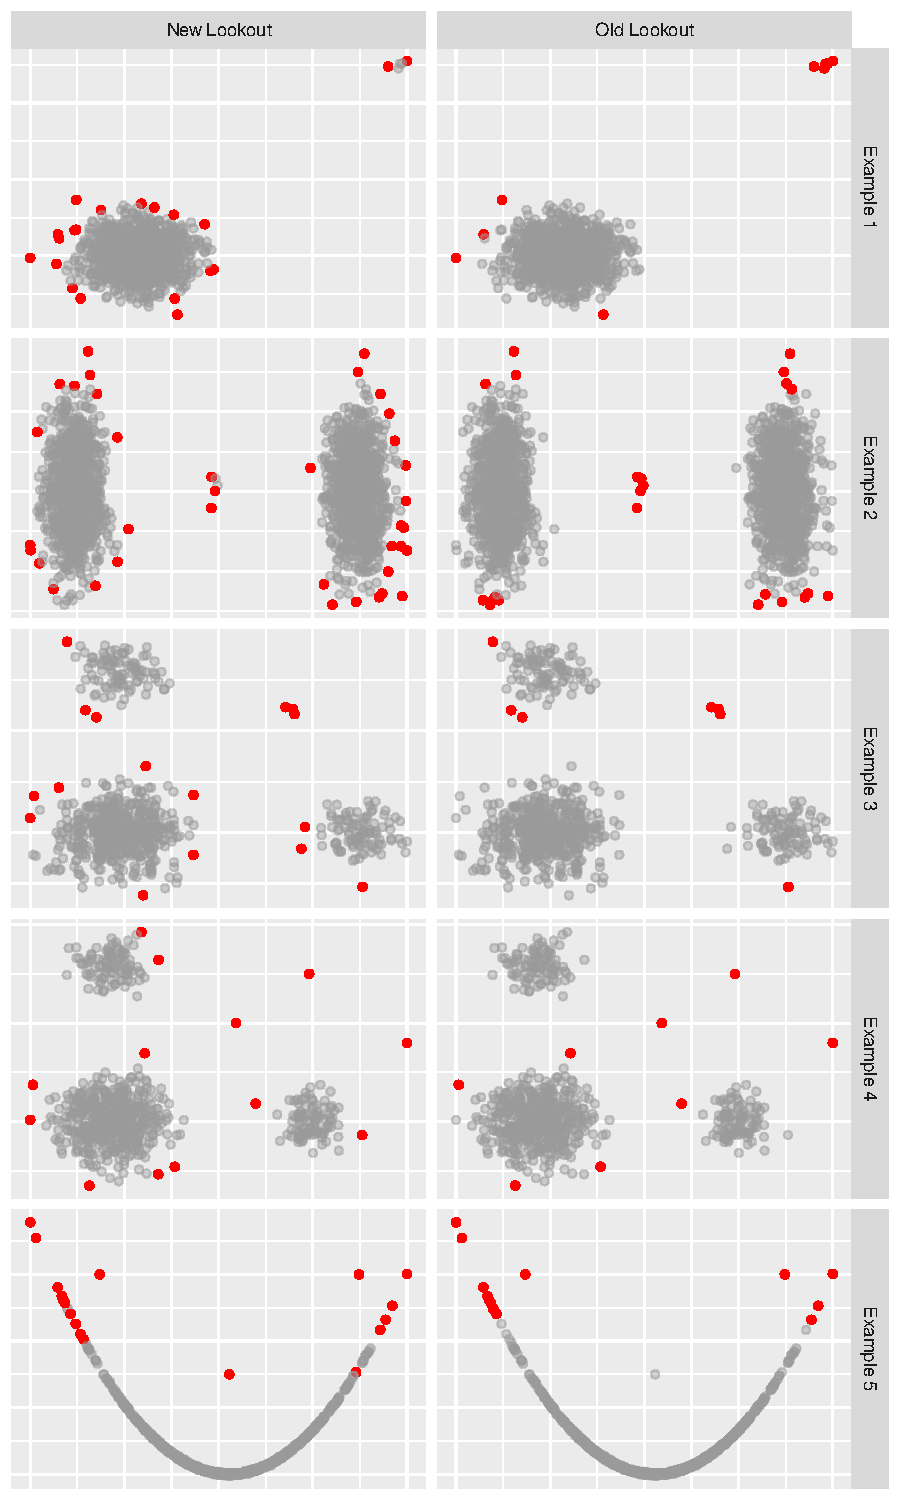
\includegraphics[width=0.74\linewidth]{Figures/Showcase_Examples.pdf}
  \caption{Showcase examples. Anomalies identified by the new (left) and original (right) versions of lookout are in red.}
  \label{fig:showcaseExamples}
\end{figure}

\cref{fig:showcaseExamples} applies both versions to five examples in $\R^2$, to check that the new version agrees with the original on obvious anomalies. In the first row, five anomalies lie at the top right of a standard normal sample. In the second, five anomalies lie midway between two normal clusters. In the third, a group of three anomalies lies away from three normal clusters, and in the fourth the three anomalies are spread out. In each of these four rows both versions identify all the anomalies, and the new version flags more non-anomalous points: 12, 24, 9 and 5 against 3, 17, 2 and 2 for the original. In the last row the non-anomalous points lie on a parabola and three anomalies lie off it. Neither version takes account of the geometry of the curve, so this example is difficult. The new version identifies all three anomalies and the original two, and they flag 13 and 9 points on the curve. Overall, the new version is more sensitive to anomalies and produces more false positives. Its false positives tend to be in regions of low density, which is consistent with our definition of an anomaly.

\subsection{Sensitivity to the bandwidth}\label{sec:ablationsupp}

Section 2.3 of the main paper argues that the bandwidth should be of the order of the spacing in the tails, and that neither the constant nor MISE-optimality matters much. To check this, we repeat Experiments 1, 2 and 3 of the main paper, and Experiment S1, with the bandwidth $h_n$ multiplied by $1/4$, $1/2$, $2$ and $4$, and with $h_n$ replaced by the bandwidth $h_{\text{opt}}$ of Table 1 of the main paper, the AMISE-optimal bandwidth for the Epanechnikov kernel and a standard normal density, computed for the standardized data. Everything else in Algorithm 2 of the main paper is unchanged. In Experiment 2 we use $n\in\{1000, 2000, 4000\}$ and the exact leave-one-out estimate, so that the truncated sum of Section 3 of the main paper does not affect the results at large multiples of $h_n$. Each setting is replicated ten times. \cref{fig:ablation} reports the area under the ROC curve computed from the anomaly scores, and the true and false positive rates at $\alpha=0.01$.

The ranking of the observations is insensitive to the bandwidth. The area under the ROC curve is almost the same for every bandwidth from $h_n/2$ to $4h_n$ in all four experiments, apart from three iterations of Experiment 3 at $4h_n$. At $h_n/4$ it is lower in Experiments 2 and S1, and in Experiment 3 from the fourth iteration. The threshold is more sensitive. At $h_n$ the false positive rate is between $0.005$ and $0.013$ in the four experiments, close to the nominal $\alpha=0.01$. At $h_n/4$ it is between $0.05$ and $0.27$, because observations with no other observation inside the kernel support have a leave-one-out estimate of zero and are all declared anomalous; in Experiment 3 the GPD could not be fitted in 10 of the 100 runs at $h_n/4$. Doubling or quadrupling the bandwidth keeps the false positive rate at or below the nominal level and, in Experiments 1 and 2, lowers the true positive rate, because the estimate at an isolated observation then includes contributions from the bulk of the sample. In Experiments 2 and S1, with normal observations in two dimensions, $h_{\text{opt}}$ is on average about $h_n$ and $0.75h_n$ respectively, and gives similar results. In Experiment 1, with gamma observations, it is about a third of $h_n$ and gives a false positive rate of $0.02$. In Experiment 3, where $m=6$, it is about a quarter of $h_n$; the GPD could not be fitted in 73 of the 100 runs, because more than $10\%$ of the observations had no other observation inside the kernel support, and in the remaining runs the false positive rate averaged $0.34$. As described in Section 2.3 of the main paper, in moderate dimensions a bandwidth chosen for the bulk of the distribution is too small for the tails.

\begin{figure}[!p]
  \centering
  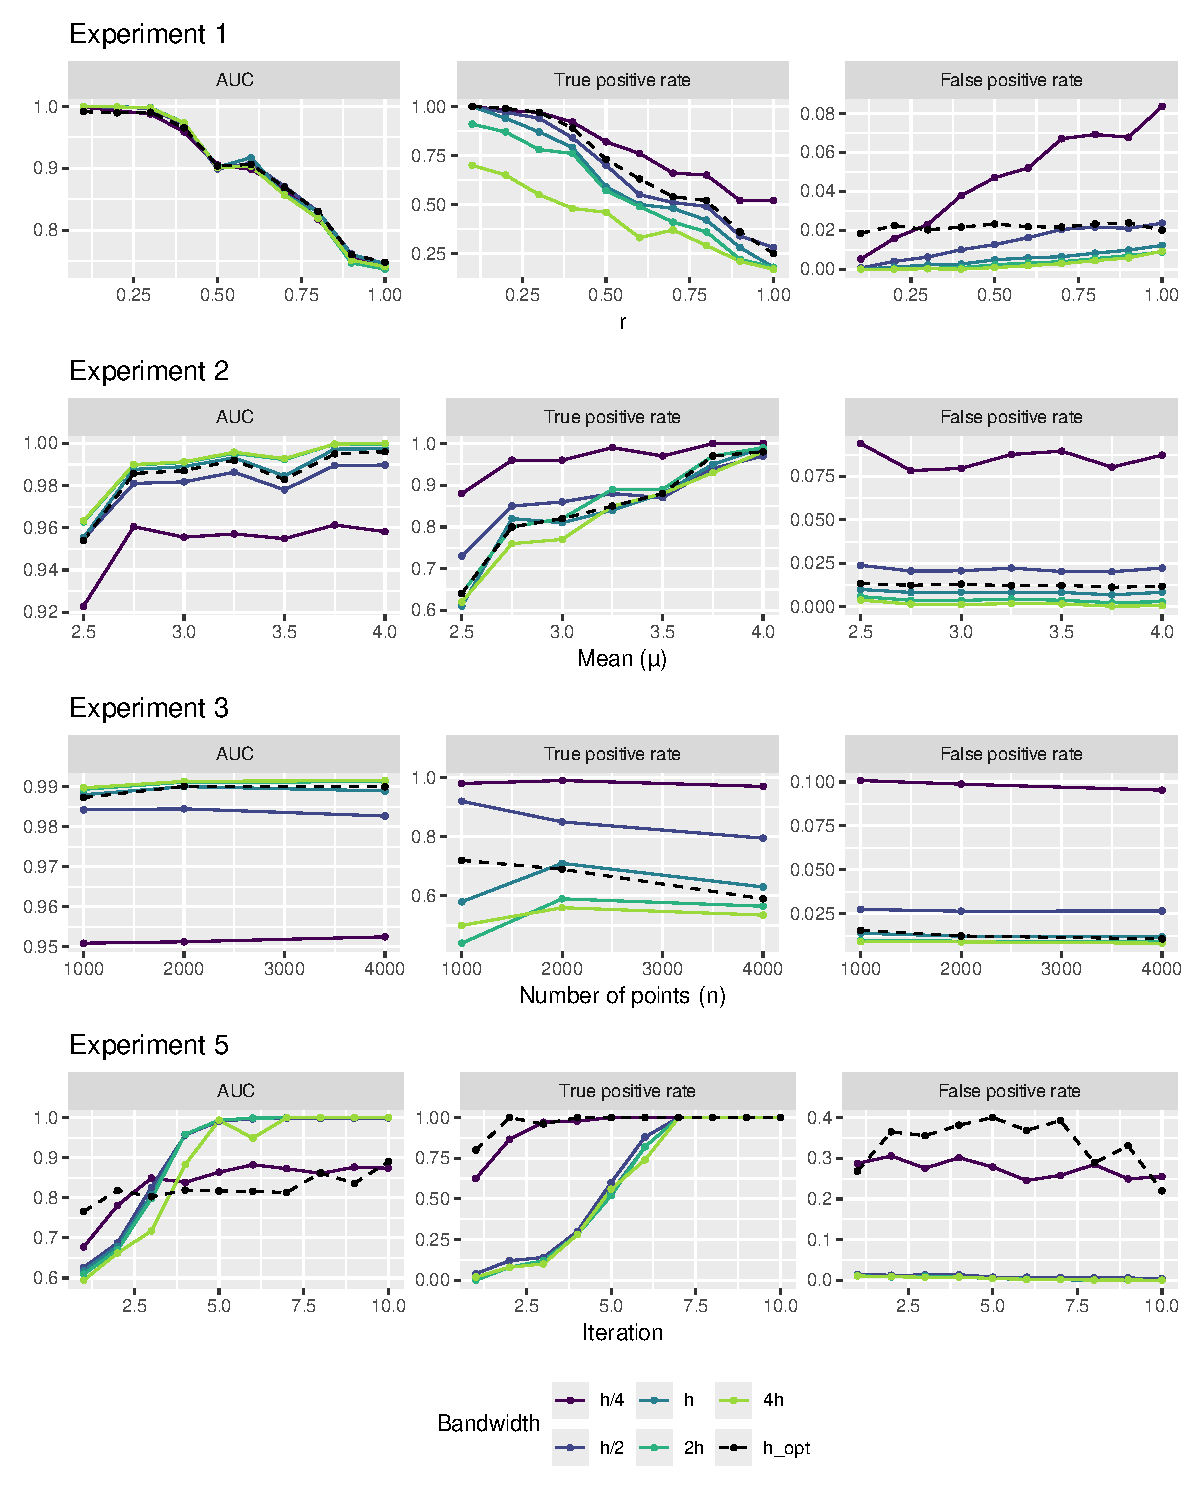
\includegraphics[width=0.84\linewidth]{Figures/bandwidth_ablation.pdf}
  \caption{Sensitivity of the new version of lookout to the bandwidth in Experiments 1, 2 and 3 of the main paper and Experiment S1: mean over ten replications of the area under the ROC curve and of the true and false positive rates, with the minimum spanning tree bandwidth $h_n$ multiplied by $1/4$, $1/2$, $1$, $2$ and $4$, and with the AMISE-optimal bandwidth $h_{\text{opt}}$ of Table 1 of the main paper (dashed).}
  \label{fig:ablation}
\end{figure}
